\documentclass[12pt]{article}
\usepackage{fullpage}
\usepackage{hyperref}
\usepackage{natbib}
\usepackage{tikz}
\usepackage{amssymb,amsmath}
\DeclareMathOperator*{\minimize}{minimize}

\begin{document}

\title{GFPOP for ECG data}
\author{Toby Dylan Hocking}
\maketitle


\begin{figure}
  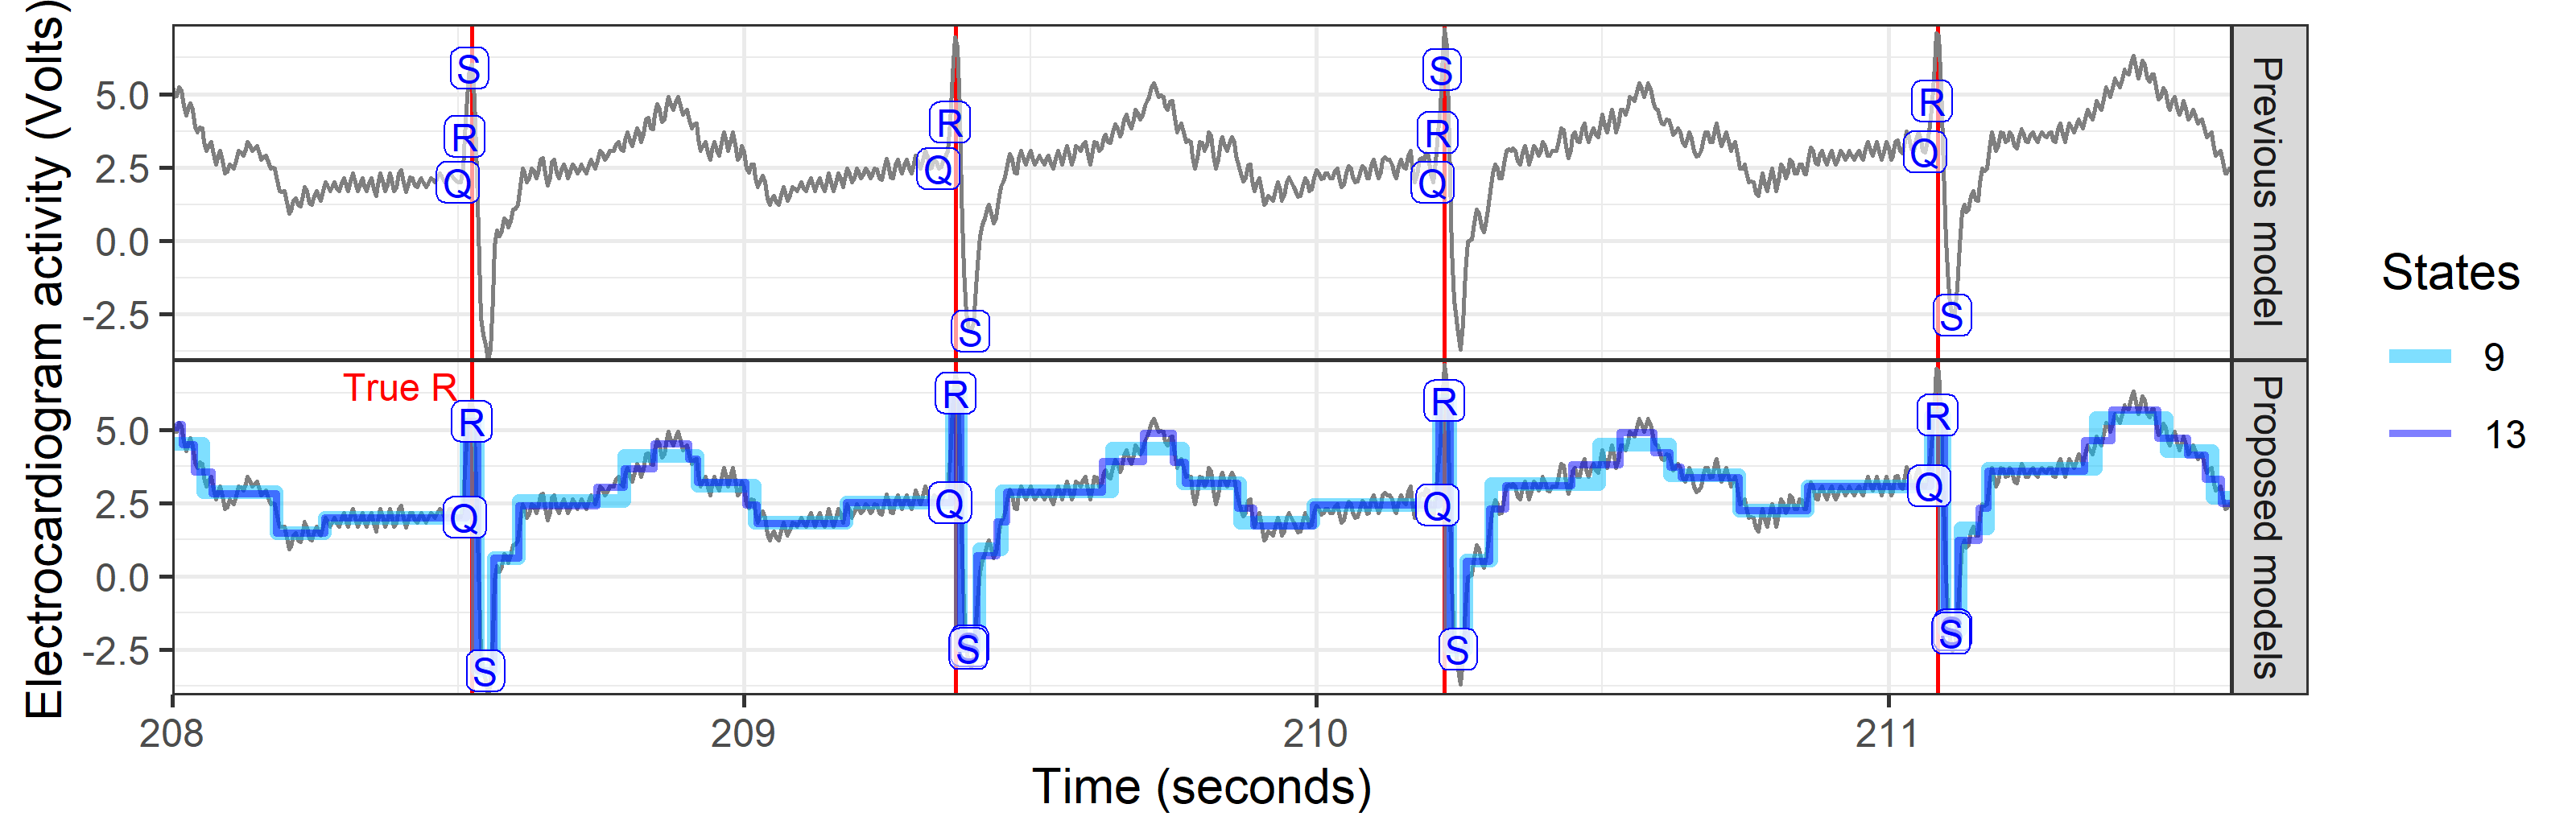
\includegraphics[width=\textwidth]{figure-two-ecg-graphs-data}

  
\definecolor{deepskyblue}{RGB}{0,191,255}
\begin{tikzpicture}[->,>=latex,shorten >=1pt,auto,node distance=1.3cm,
      thick,main node/.style={circle,draw}]
 \node[main node, fill=white!50!deepskyblue, text=blue] (b)  {b};
 \node[main node, fill=white!50!deepskyblue, text=blue] (Q) [right of=b] {Q};
 \node[main node, fill=white!50!deepskyblue, text=blue] (R) [right of=Q] {R};
 \node[main node, fill=white!50!deepskyblue, text=blue] (S) [right of=R] {S};
 \node[main node, fill=white!50!deepskyblue, text=blue] (x1) [right of=S] {x1};
 \node[main node, fill=white!50!deepskyblue, text=blue] (x2) [right of=x1] {x2};
 \node[main node, fill=white, text=blue] (x3) [right of=x2] {x3};
 \node[main node, fill=white, text=blue] (x4) [right of=x3] {x4};
 \node[main node, fill=white!50!deepskyblue, text=blue] (y1) [right of=x4] {y1};
 \node[main node, fill=white!50!deepskyblue, text=blue] (y2) [right of=y1] {y2};
 \node[main node, fill=white, text=blue] (y3) [right of=y2] {y3};
 \node[main node, fill=white, text=blue] (y4) [right of=y3] {y4};
 \node[main node, fill=white!50!deepskyblue, text=blue] (y5) [right of=y4] {y5};
 
\path[every node/.style={font=\sffamily\small}]
 (b) edge [bend left] node [above] {$\lambda, \downarrow$} node [below] {\scriptsize } (Q)
 (Q) edge [bend left] node [above] {$0, \uparrow$} node [below] {\scriptsize 2} (R)
 (R) edge [bend left] node [above] {$0, \downarrow$} node [below] {\scriptsize 5} (S)
 (S) edge [bend left] node [above] {$0, \uparrow$} node [below] {\scriptsize 2} (x1)
 (x1) edge [bend left] node [above] {$0, \uparrow$} node [below] {\scriptsize 1} (x2)
 (x2) edge [bend left] node [above] {$0, \uparrow$} node [below] {\scriptsize } (x3)
 (x3) edge [bend left] node [above] {$0, \uparrow$} node [below] {\scriptsize } (x4)
 (x4) edge [bend left] node [above] {$0, \uparrow$} node [below] {\scriptsize } (y1)
 (y1) edge [bend left] node [above] {$0, \downarrow$} node [below] {\scriptsize } (y2)
 (y2) edge [bend left] node [above] {$0, \downarrow$} node [below] {\scriptsize } (y3)
 (y3) edge [bend left] node [above] {$0, \downarrow$} node [below] {\scriptsize } (y4)
 (y4) edge [bend left] node [above] {$0, \downarrow$} node [below] {\scriptsize } (y5)
 (y5) edge [bend left, looseness=0.4] node [above] {$0, \uparrow$} node [below] {\scriptsize } (b)
 ;
\end{tikzpicture}

  \caption{\label{fig:ecg} In these electrocardiogram data, it is
    important for models (\textcolor{blue}{blue}) to accurately detect
    the QRS complex (Q is before the peak, R is the peak marked in
    \textcolor{red}{red}, S is the local minimum after the
    peak). \textbf{Top:} Previous model of \citet{PanTompkins1985}
    mistakenly predicts S at the peak. \textbf{Bottom:} proposed
    constrained changepoint model using a graph with 9 vertices
    accurately predicts R at each peak.}

\end{figure}

\bibliographystyle{abbrvnat}
\bibliography{refs}

\end{document}